%%%%%%%%%%%%%%%%%%%%%%%%%%%%%%%%%%%%%%%%%
% Beamer Presentation
% LaTeX Template
% Version 2.0 (March 8, 2022)
%
% This template originates from:
% https://www.LaTeXTemplates.com
%
% Author:
% Vel (vel@latextemplates.com)
%
% License:
% CC BY-NC-SA 4.0 (https://creativecommons.org/licenses/by-nc-sa/4.0/)
%
%%%%%%%%%%%%%%%%%%%%%%%%%%%%%%%%%%%%%%%%%

%----------------------------------------------------------------------------------------
%	PACKAGES AND OTHER DOCUMENT CONFIGURATIONS
%----------------------------------------------------------------------------------------

\documentclass[
	11pt, % Set the default font size, options include: 8pt, 9pt, 10pt, 11pt, 12pt, 14pt, 17pt, 20pt
	%t, % Uncomment to vertically align all slide content to the top of the slide, rather than the default centered
	%aspectratio=169, % Uncomment to set the aspect ratio to a 16:9 ratio which matches the aspect ratio of 1080p and 4K screens and projectors
]{beamer}

\graphicspath{{Images/}{./}} % Specifies where to look for included images (trailing slash required)

\usepackage{booktabs} % Allows the use of \toprule, \midrule and \bottomrule for better rules in tables
\usepackage{listings}

%----------------------------------------------------------------------------------------
%	SELECT LAYOUT THEME
%----------------------------------------------------------------------------------------

% Beamer comes with a number of default layout themes which change the colors and layouts of slides. Below is a list of all themes available, uncomment each in turn to see what they look like.

%\usetheme{default}
%\usetheme{AnnArbor}
%\usetheme{Antibes}
%\usetheme{Bergen}
%\usetheme{Berkeley}
%\usetheme{Berlin}
%\usetheme{Boadilla}
%\usetheme{CambridgeUS}
%\usetheme{Copenhagen}
%\usetheme{Darmstadt}
%\usetheme{Dresden}
\usetheme{Frankfurt}
%\usetheme{Goettingen}
%\usetheme{Hannover}
%\usetheme{Ilmenau}
%\usetheme{JuanLesPins}
%\usetheme{Luebeck}
%\usetheme{Madrid}
%\usetheme{Malmoe}
%\usetheme{Marburg}
%\usetheme{Montpellier}
%\usetheme{PaloAlto}
%\usetheme{Pittsburgh}
%\usetheme{Rochester}
%\usetheme{Singapore}
%\usetheme{Szeged}
%\usetheme{Warsaw}

%----------------------------------------------------------------------------------------
%	SELECT COLOR THEME
%----------------------------------------------------------------------------------------

% Beamer comes with a number of color themes that can be applied to any layout theme to change its colors. Uncomment each of these in turn to see how they change the colors of your selected layout theme.

%\usecolortheme{albatross}
%\usecolortheme{beaver}
%\usecolortheme{beetle}
%\usecolortheme{crane}
%\usecolortheme{dolphin}
%\usecolortheme{dove}
%\usecolortheme{fly}
%\usecolortheme{lily}
%\usecolortheme{monarca}
%\usecolortheme{seagull}
%\usecolortheme{seahorse}
%\usecolortheme{spruce}
%\usecolortheme{whale}
%\usecolortheme{wolverine}

%----------------------------------------------------------------------------------------
%	SELECT FONT THEME & FONTS
%----------------------------------------------------------------------------------------

% Beamer comes with several font themes to easily change the fonts used in various parts of the presentation. Review the comments beside each one to decide if you would like to use it. Note that additional options can be specified for several of these font themes, consult the beamer documentation for more information.

\usefonttheme{default} % Typeset using the default sans serif font
%\usefonttheme{serif} % Typeset using the default serif font (make sure a sans font isn't being set as the default font if you use this option!)
%\usefonttheme{structurebold} % Typeset important structure text (titles, headlines, footlines, sidebar, etc) in bold
%\usefonttheme{structureitalicserif} % Typeset important structure text (titles, headlines, footlines, sidebar, etc) in italic serif
%\usefonttheme{structuresmallcapsserif} % Typeset important structure text (titles, headlines, footlines, sidebar, etc) in small caps serif

%------------------------------------------------

%\usepackage{mathptmx} % Use the Times font for serif text
\usepackage{palatino} % Use the Palatino font for serif text

%\usepackage{helvet} % Use the Helvetica font for sans serif text
\usepackage[default]{opensans} % Use the Open Sans font for sans serif text
%\usepackage[default]{FiraSans} % Use the Fira Sans font for sans serif text
%\usepackage[default]{lato} % Use the Lato font for sans serif text
\usepackage{hyperref}
%----------------------------------------------------------------------------------------
%	SELECT INNER THEME
%----------------------------------------------------------------------------------------

% Inner themes change the styling of internal slide elements, for example: bullet points, blocks, bibliography entries, title pages, theorems, etc. Uncomment each theme in turn to see what changes it makes to your presentation.

%\useinnertheme{default}
\useinnertheme{circles}
%\useinnertheme{rectangles}
%\useinnertheme{rounded}
%\useinnertheme{inmargin}

%----------------------------------------------------------------------------------------
%	SELECT OUTER THEME
%----------------------------------------------------------------------------------------

% Outer themes change the overall layout of slides, such as: header and footer lines, sidebars and slide titles. Uncomment each theme in turn to see what changes it makes to your presentation.

%\useoutertheme{default}
%\useoutertheme{infolines}
%\useoutertheme{miniframes}
%\useoutertheme{smoothbars}
%\useoutertheme{sidebar}
%\useoutertheme{split}
%\useoutertheme{shadow}
%\useoutertheme{tree}
%\useoutertheme{smoothtree}

%\setbeamertemplate{footline} % Uncomment this line to remove the footer line in all slides
%\setbeamertemplate{footline}[page number] % Uncomment this line to replace the footer line in all slides with a simple slide count

%\setbeamertemplate{navigation symbols}{} % Uncomment this line to remove the navigation symbols from the bottom of all slides

%----------------------------------------------------------------------------------------
%	PRESENTATION INFORMATION
%----------------------------------------------------------------------------------------

\title[Inverse shortest paths in directed acyclic graphs]{Inverse shortest paths in directed acyclic graphs} % The short title in the optional parameter appears at the bottom of every slide, the full title in the main parameter is only on the title page

\subtitle{Presentation for KLAIM 2023} % Presentation subtitle, remove this command if a subtitle isn't required

\author[Sven O. Krumke, Florian Dahms, Orges Leka]{Sven O. Krumke, Florian Dahms, Orges Leka} % Presenter name(s), the optional parameter can contain a shortened version to appear on the bottom of every slide, while the main parameter will appear on the title slide

\institute[TH-Bingen]{Technische Hochschule Bingen \\ \smallskip \textit{o.leka@th-bingen.de}} % Your institution, the optional parameter can be used for the institution shorthand and will appear on the bottom of every slide after author names, while the required parameter is used on the title slide and can include your email address or additional information on separate lines

\date[\today]{Presentation \\ \today} % Presentation date or conference/meeting name, the optional parameter can contain a shortened version to appear on the bottom of every slide, while the required parameter value is output to the title slide

%----------------------------------------------------------------------------------------

\begin{document}

%----------------------------------------------------------------------------------------
%	TITLE SLIDE
%----------------------------------------------------------------------------------------

\begin{frame}
	\titlepage % Output the title slide, automatically created using the text entered in the PRESENTATION INFORMATION block above
\end{frame}

%----------------------------------------------------------------------------------------
%	TABLE OF CONTENTS SLIDE
%----------------------------------------------------------------------------------------

% The table of contents outputs the sections and subsections that appear in your presentation, specified with the standard \section and \subsection commands. You may either display all sections and subsections on one slide with \tableofcontents, or display each section at a time on subsequent slides with \tableofcontents[pausesections]. The latter is useful if you want to step through each section and mention what you will discuss.

\begin{frame}
	\frametitle{Overview} % Slide title, remove this command for no title
	
	\tableofcontents % Output the table of contents (all sections on one slide)
	%\tableofcontents[pausesections] % Output the table of contents (break sections up across separate slides)
\end{frame}

%----------------------------------------------------------------------------------------
%	PRESENTATION BODY SLIDES
%----------------------------------------------------------------------------------------

\section{Introduction} % Sections are added in order to organize your presentation into discrete blocks, all sections and subsections are automatically output to the table of contents as an overview of the talk but NOT output in the presentation as separate slides

%------------------------------------------------


%------------------------------------------------
\subsection{Problem definition of Burton und Toint 1992}
\begin{frame}
	\frametitle{Problem definition of Burton und Toint 1992}
	
	\begin{itemize}
	    \item Given: A directed graph $G = (V,E)$,  costs $c$ on the edges, a set $P$ of paths.
            \item we are searching for: costs $\hat{c}$ on the edges, such that:
            \item $\hat{c}:= \operatorname{argmin}_{\hat{c}} \sum_{(u,v)\in E} (c(u,v)-\hat{c}(u,v))^2$
            \item under constraint: $\forall p \in P$ ist $p$ is a shortest path under $\hat{c}$
	\end{itemize}

\end{frame}


\begin{frame}
	\frametitle{possible Application:}
	
	\begin{itemize}
	    \item given: A directed graph $G = (V,E)$,  costs $c$ on the edges, a set $P$ of paths.
            \item vertices correspond here to railway routes so called 'Fahrwege'
            \item edges correspond to connections of Fahrwege
            \item Set of paths $p \in P$ corresponds to paths from given schedules which were constructed manually
	\end{itemize}

\end{frame}

\subsection{Heuristic Idea}
\begin{frame}
	\frametitle{Heuristic Idea}
	
	\begin{itemize}
	    \item Divide the problem of Burton and Toint into two tasks:
            \item Desired: Costs $\hat{c}$ on the edges such that:
            \item 1. For all $p \in P$, $p$ is a shortest path under $\hat{c}$
            \item 2. Modify $\hat{c}$ to $c^*(u,v):= \hat{c}(u,v)+h_v-h_u$, where:
            \item  $c^*:=\operatorname{argmin}_{h} \sum_{(u,v)\in E} (c(u,v)-(\hat{c}(u,v)+h_v-h_u))^2$

	\end{itemize}

\end{frame}

\begin{frame}
      \frametitle{1st Step in the Heuristic Idea: Straight Line as a Shortest Line}
	\begin{figure}
		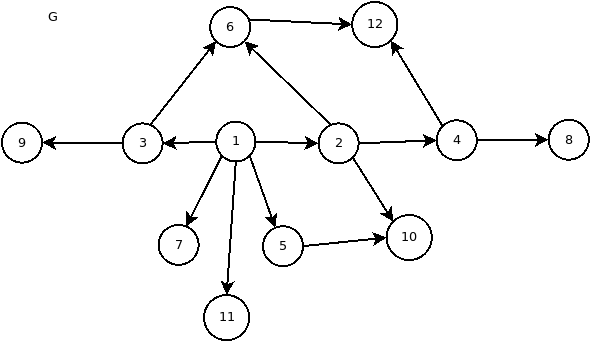
\includegraphics[width=0.8\linewidth]{Figur01.png}
		\caption{Example graph G}
	\end{figure}
\end{frame}

\begin{frame}
      \frametitle{1st Step in the Heuristic Idea: Straight Line as a Shortest Line}
	\begin{figure}
		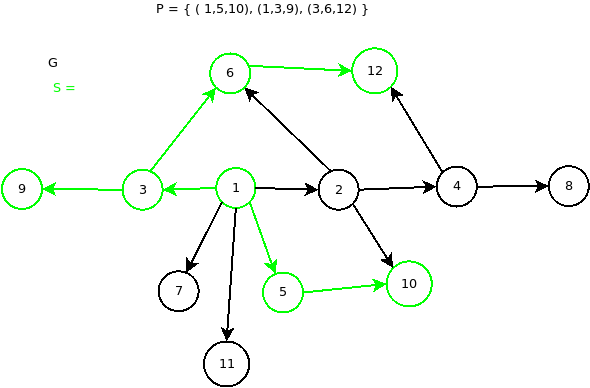
\includegraphics[width=0.8\linewidth]{Figur02.png}
		\caption{Preserve prescribed paths in subgraph S}
	\end{figure}
\end{frame}


\begin{frame}
      \frametitle{1st Step in the Heuristic Idea: Straight Line as a Shortest Line}
	\begin{figure}
		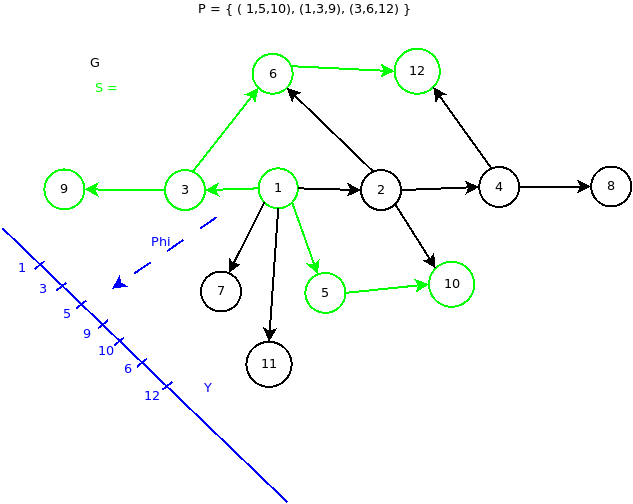
\includegraphics[width=0.8\linewidth]{Figur03.png}
		\caption{Nodes projected onto straight line according to topological sorting}
	\end{figure}
\end{frame}


\begin{frame}
      \frametitle{1st Step in the Heuristic Idea: Straight Line as a Shortest Line}
	\begin{figure}
		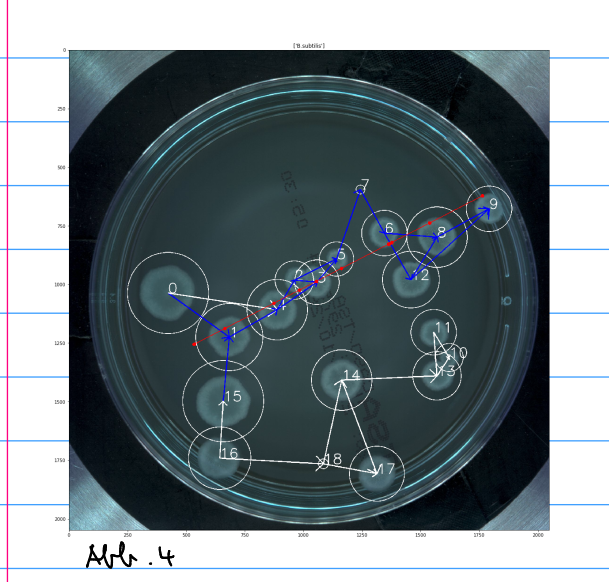
\includegraphics[width=0.6\linewidth]{Figur04.png}
		\caption{blue=Prescribed paths, red=Projection line, white=Graph}
	\end{figure}
\end{frame}

\begin{frame}
      \frametitle{2nd Step in the Heuristic Idea: Use Potential Function $h_v$ to Modify Costs}
      Given: \\
\begin{itemize}
  \item $\mathbf{c}(u,v):=$ Currently used costs 
  \item $\hat{c}(u,v):=$ Shortest path costs calculated in the 1st step
\end{itemize}
\end{frame}

\begin{frame}
      \frametitle{2nd Step in the Heuristic Idea: Use Potential Function $h_v$ to Modify Costs}
      Desired: Potential function $h: V \rightarrow \mathbf{R}$ that minimizes $(*):$\\

$$ (*): \min_{h} \sum_{(u,v) \in E} (\mathbf{c}(u,v)-(\hat{c}(u,v)+h_v-h_u))^2 $$\\
  $$ \text{ and } \gamma(u,v):= \hat{c}(u,v) + h_v-h_u\ge^! 0$$

\end{frame}

\begin{frame}
      \frametitle{2nd Step in the Heuristic Idea: Use Potential Function $h_v$ to Modify Costs}
      Two Ideas: \\
      (i) Formulate (*) as an optimization problem and solve it with an optimizer \\
      (ii) Use a heuristic to solve (*) quickly (Idea from Johnson's or Surballee's Algorithm)
\end{frame}

\section{Extension using Kernel Trick}
\begin{frame}
      \frametitle{Extension using Kernel Trick}
      Observation:\\
      The heuristic method only uses distances and inner products in the calculations\\
      This inner product can be replaced by a positive definite kernel $k$\\
      Distance: $d(x,y) = \sqrt{k(x,x)+k(y,y)-2k(x,y)}$
      
\end{frame}

\begin{frame}
      \frametitle{Extension using Kernel Trick}
      Advantage:\\
      Properties of routes such as:
      \begin{itemize}
       \item Number of switches
       \item Number of intersections
       \item Length
       \item Passenger exit yes/no
       \item Maximum speed
     \end{itemize}
     can be taken into account in the cost calculation of the distance function.\\
     
     Different distance functions could be defined and empirically tested for suitability.
       
\end{frame}

\section{Examples}
\subsection{Example Calculation}

\begin{frame}
	\frametitle{Graph G with Distance Costs}
	
	$c(u,v) := \sqrt{|\min(u,u)+\min(v,v)-2 \cdot \min(u,v)|} = \sqrt{|u-v|}$
	
	\begin{figure}
		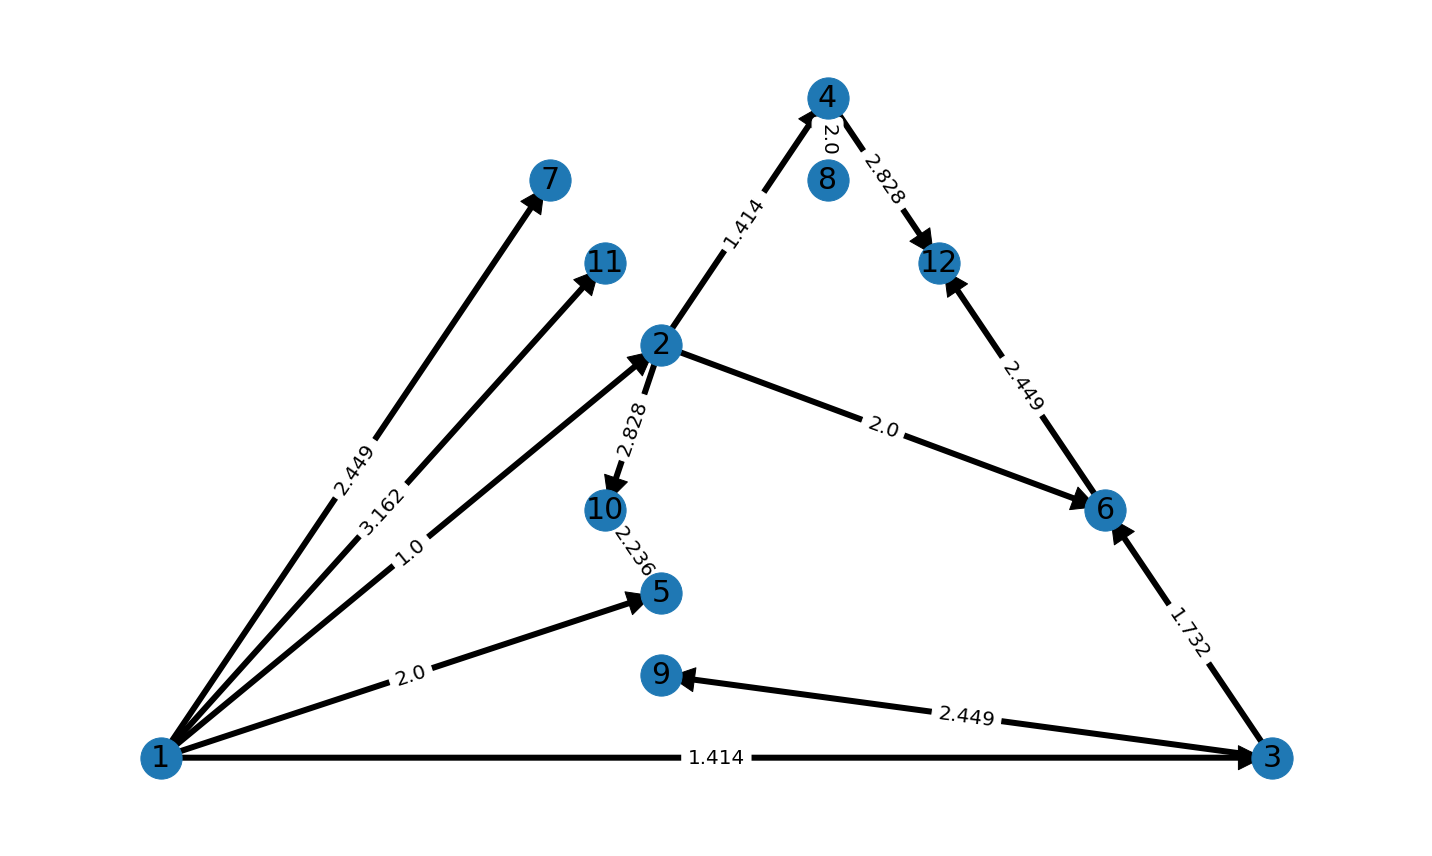
\includegraphics[width=0.8\linewidth]{graphG.png}
		\caption{Graph G with Distance Costs}
	\end{figure}
\end{frame}

\begin{frame}
	\frametitle{Graph H with Currently Used Costs}
	
	\begin{figure}
		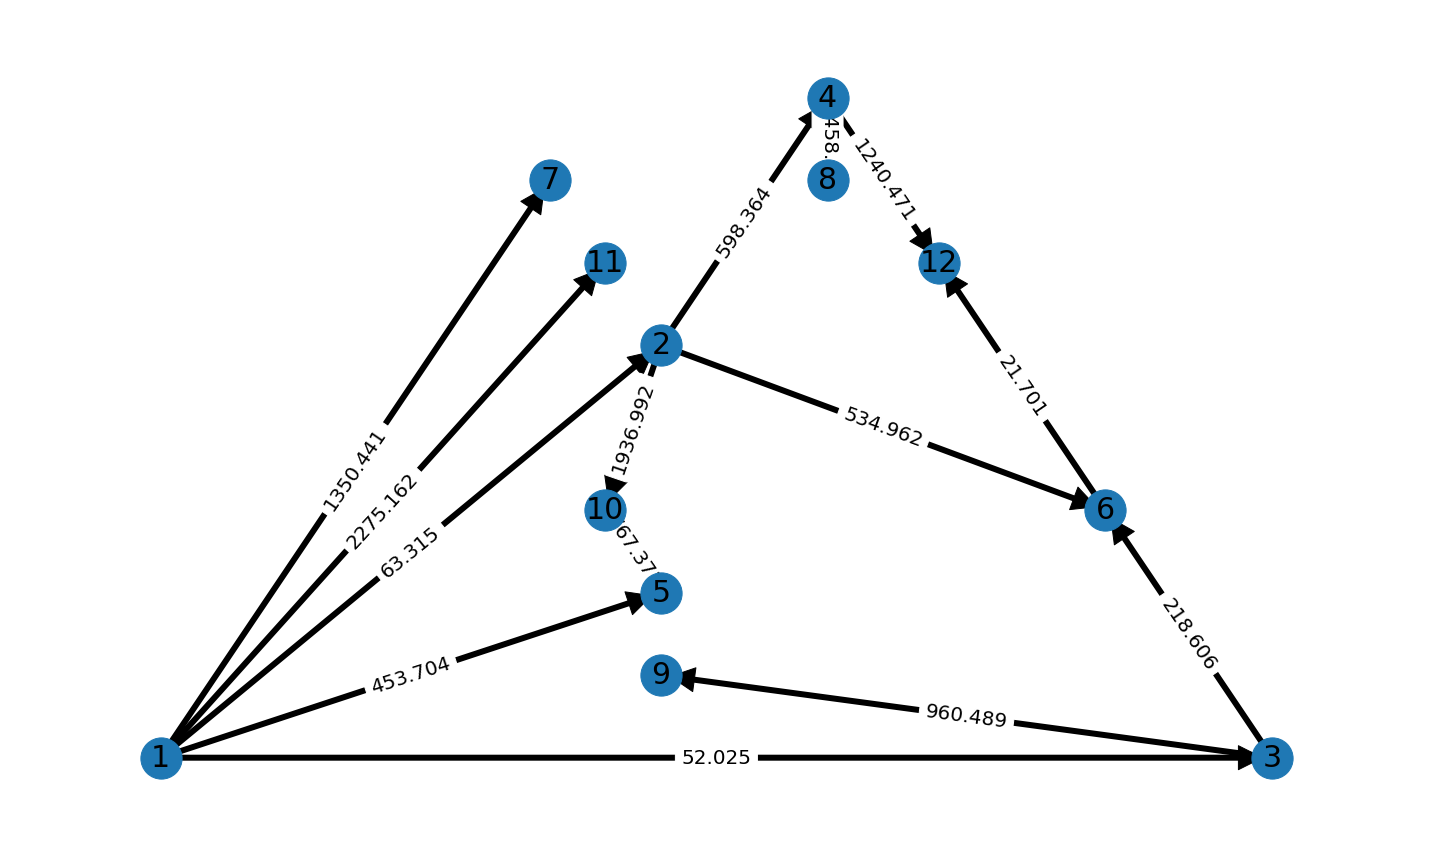
\includegraphics[width=0.8\linewidth]{graphH.png}
		\caption{Graph H with Currently Used Costs}
	\end{figure}
\end{frame}


\begin{frame}
	\frametitle{Graph I with Costs for Shortest Paths}
	
	\begin{figure}
		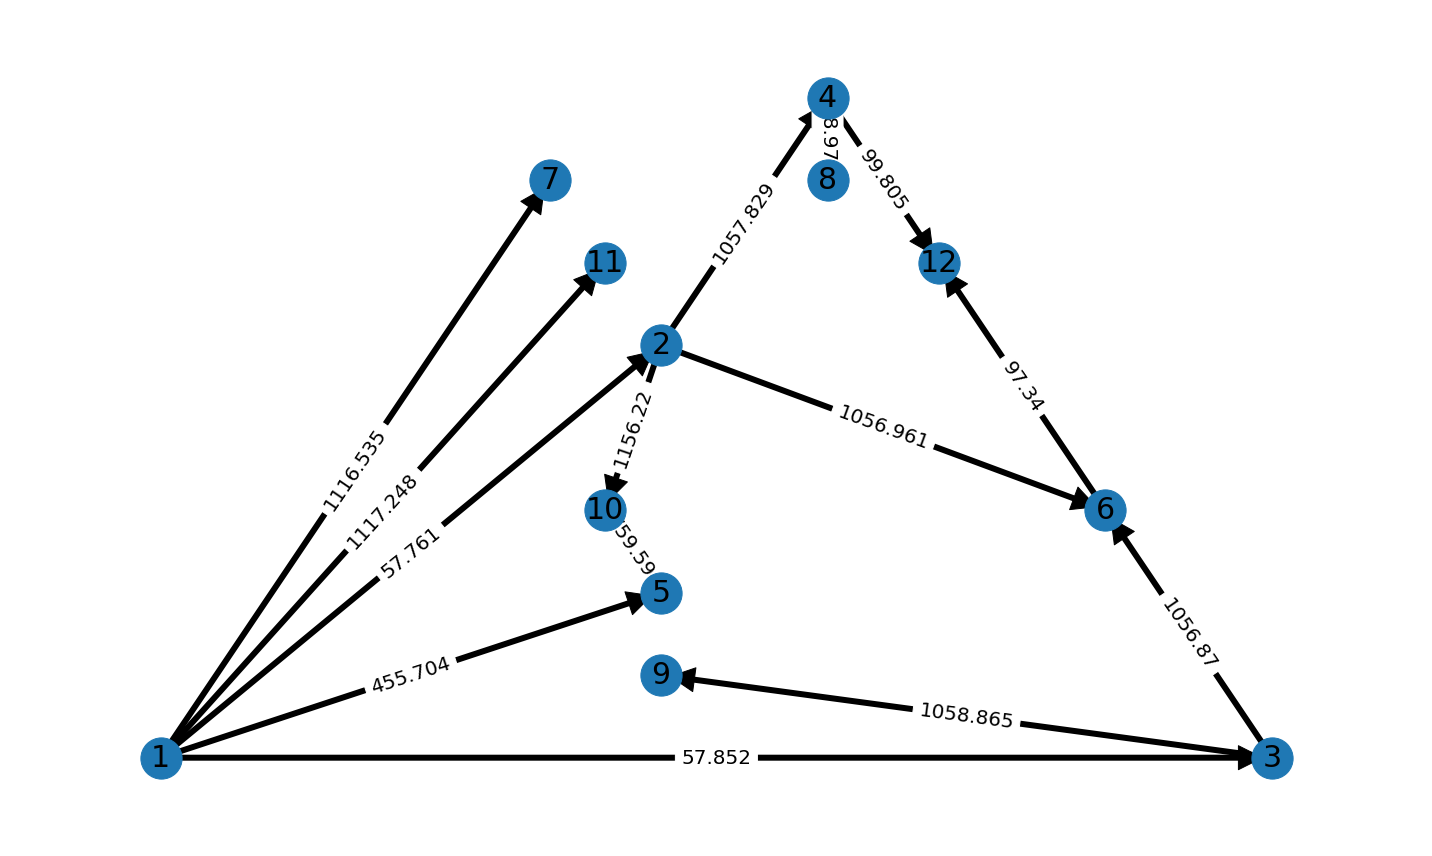
\includegraphics[width=0.8\linewidth]{graphI.png}
		\caption{Graph I with Costs for Shortest Paths}
	\end{figure}
\end{frame}

\begin{frame}
      \frametitle{Prescribed Paths}
paths =  [(1, 2, 6, 12), (1, 3, 6, 12)] \\


shortest path as required: (1, 2, 6, 12) 1212.06 1212.06 \\
shortest path as required: (1, 3, 6, 12) 1212.06 1212.06 \\
not a shortest path as required: (1, 2, 4, 12) 1215.39 1212.06      
\end{frame}      

\section{Runtimes 1st Step}
\begin{frame}
    \frametitle{Runtimes for the 1st Step in the Heuristic}
	\begin{figure}
		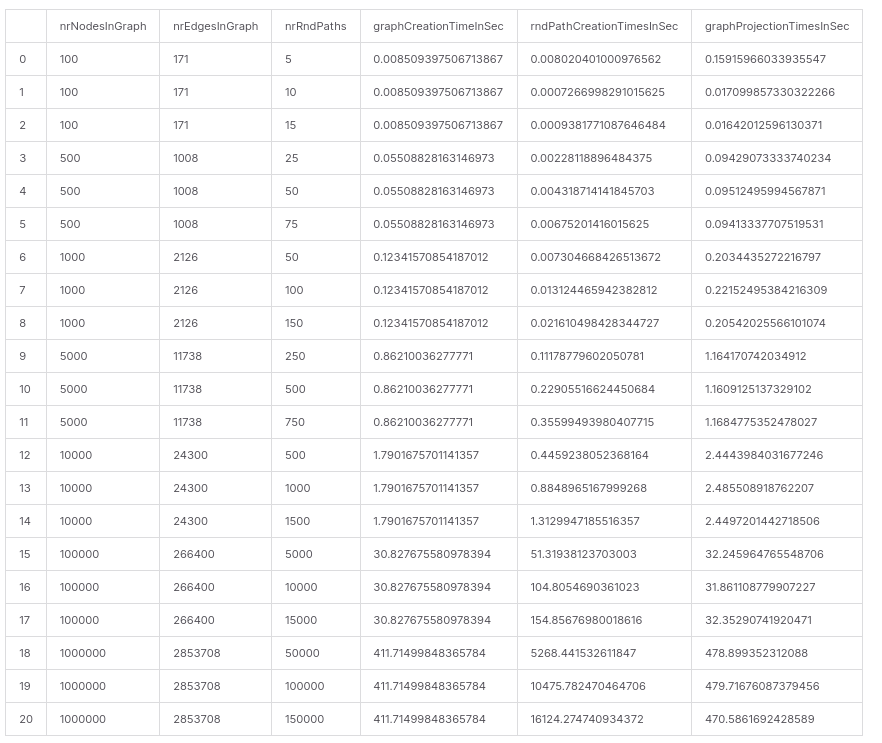
\includegraphics[width=0.6\linewidth]{ErgebnisHeuristik1Schritt.png}
		\caption{Result: Heuristic 1st Step, Runtimes in seconds}
	\end{figure}
    
\end{frame}

%------------------------------------------------


%------------------------------------------------

%------------------------------------------------


%----------------------------------------------------------------------------------------
%	CLOSING SLIDE
%----------------------------------------------------------------------------------------

\begin{frame}[plain] % The optional argument 'plain' hides the headline and footline
	\begin{center}
		{\Huge Thank you for your attention}
		
		\bigskip\bigskip % Vertical whitespace
		
		{\LARGE Any Questions? Comments?}
		
		\bigskip
		Code and paper may be found here: https://github.com/githubuser1983/klaim2023
	\end{center}
\end{frame}
%----------------------------------------------------------------------------------------

\end{document} 
